% Theorems, lemmas etc.

\documentclass[../main.tex]{subfiles}
\graphicspath{{\subfix{../images/}}}

\begin{document}

\part{MISC}

数学基本思想:\\
抽象能力:会在错综复杂的事物中把握本质\\
推理能力:会在杂乱无章的事物中理清头绪\\
建模能力:会在千头万绪的事物中发现规律

数学四大基本思想:\\
函数与方程、数形结合、分类讨论和转化与化归(复杂或未知的问题,通过一定的变换,最终归结为已知或更容易解决的问题的思维方法)

数学基本方法:\\
数形结合、分类讨论、换元、数学归纳法、反证法、类比

数域(域:field):\\
指一个数集,它对加法、减法、乘法和除法(除数不为零)运算是封闭的,并且包含$0$和$1$\\
换句话说,对数域中任意两个数进行这四种基本运算,其结果仍然属于这个数域。\\
常见的数域包括有理数域(Q)、实数域(R) 和复数域(C)\\
一个集合成为数域,需满足以下条件:\\
1. 包含0和1:数域中必须有加法单位元0和乘法单位元1\\
2. 封闭性:加法和减法封闭;乘法封闭;除法封闭\\
非数域例子:自然数集和整数集,不构成数域,因为除法运算不封闭,例如$2/3$不属于自然数或者整数

丢番图方程:\\
丢番图方程,又称为不定方程(Diophantine equation), Diophantus is a Greek mathematician\\
丢番图的研究在数论中占有重要地位,如丢番图方程、丢番图集合、丢番图逼近等都是数学的重要领域

最大公约数:GCD(Greatest Common Divisor) or HCF:(Highest Common Factor).\\
e.g. $gcd(3,9)=3$ , $gcd(-3,9)=3$

$0!$规定为$1$

\part{Part1}

\section{算术基本定理}
Fundamental theorem of arithmetic, also called unique factorization theorem(正整数唯一分解定理), or prime factorization theorem.

\begin{mdframed}
\textbf{STATEMENT}:\\
Every positive integer $n>1$ can be represented in exactly one way as a product of prime powers:\\
$ n = p_1^{n_1}p_2^{n_2}\cdots p_k^{n_k} = \prod_{i=1}^kp_i^{n_i}$, where $p_1<p_2<p_3\ldots <p_k$ are primes,and $n_i$ are positive integers.
\end{mdframed}
Since $a^0=1$, any positive integer can be uniquely represented as an infinite product taken over all the positive prime numbers, as
\[
n = 2^{n1}3^{n2}5^{n3}7^{n4}\cdots = \prod_{i=1}^{\infty}P_i^{n_i}
\]

每个大于1的自然数,要么本身就是素数,要么可以写为2个或以上的素数的积,而且这些素因子按大小排列之后,写法仅有一种方式。\\
例如: $ 1200 = 2^4\cdot 3 \cdot 5^2$

此定理是初等数论中一个基本定理,也是许多其他定理的逻辑支撑点和出发点。\textbf{它把对自然数的研究转化为对其最基本的元素——素数的研究}

由两部分组成:\\
1.分解存在性\\
2.分解唯一性,即若不考虑排列顺序,正整数分解为素数乘积的方式是唯一的

这个定理也是$1$不是质数的主要原因, if $1$ is prime,$2=2\cdot 1=2\cdot 1\cdot 1=\ldots $

等价命题:\\
If a prime divides the product of two integers, then it must divide at least one of these integers.That is:\\
If Prime $P|ab$, then, either $P|a$ or $P|b$ \todo{???}

Proof:

1. Existence\\
用反证法:假设存在大于$1$的自然数不能写为素数的乘积,把最小的那个称为$n$\\
n不可为素数,因为$n=n$,可以写成素数的成绩,因此$n$一定是合数,而每个合数都可以分解为两个严格小于自身而大于$1$的自然数的乘积。设$n=a\times b$,根据假设,$n$是最小的不能写为素数乘积的自然数,$a<n, b<n$,所以$a=p_1p_2\times p_n, b=q_1q_2\cdots q_n$, and $n=ab=p_1p_2\cdots p_nq_1q_2\cdots q_n$可以写为素数的乘积,由此产生矛盾,故大于$1$的自然数必可以写为素数的乘积

2. Uniqueness\\
欧几里得引理:if $p|ab$, either $p|a$ or $p|b$

\todo{todo...}

\section{代数基本定理}
Fundamental theorem of algebra, Also called "d'Alembert–Gauss theorem"
\begin{mdframed}
  \textbf{STATEMENT}:\\
  Every non-constant single-variable polynomial with complex coefficients has at least one complex root.任何一个复系数的一元$n$ 次多项式方程($n\geq 1$),至少有一个复数根。
\end{mdframed}
\begin{mdframed}
  \textbf{COROLLARY}:\\
  任何一个非零的一元 n 次复系数多项式,都正好有 n 个复数根(重根视为多个根)。
\end{mdframed}

有时候这个定理描述为:任何一个非零的一元n次复系数多项式,都正好有$n$个复数根(重根视为多个根)。但实际上,是“至少有一个根的”直接结果,因为把多项式除以它的线性因子可以推出。也就是说,任何一个$n$次多项式,都可以因式分解为$n$个复系数一次多项式的乘积(根据多项式除法\todo{Proof?})。

\textbf{意义}:复数域是代数封闭的(该定理是代数学和近世代数中的一个基础性结论);保证了任何复系数多项式方程在复数域内总有解,并能完全因式分解为一次因式(即 \(n\) 次多项式有 \(n\) 个复数根); It's the basic connection between algebra and geometry\todo{?}

尽管这个定理被命名为“代数基本定理”,但它还没有纯粹的代数证明,许多数学家都相信这种证明不存在。另外,它也不是最基本的代数定理;因为在那个时候,代数基本上就是关于解实系数或复系数多项式方程,所以才被命名为代数基本定理。

所有的证明都包含了一些数学分析,至少是实数或复数函数的连续性概念。有些证明也用到了可微函数,甚至是解析函数。

\section{多项式除法、多项式余式定理}
Polynomial division, Polynomial remainder theorem
\begin{flalign*}
  \frac{P(x)}{D(x)} = Q(x)+\frac{R(x)}{D(x)} \Rightarrow P(x)=D(x)Q(x)+R(x)&&
\end{flalign*}

If $D(x)=x-a$, then $P(x)=(x-a)Q(x)+R(x) = (x-a)Q(x)+r$\\
根据定义,$R(x)$的次数小于$1$, so $R(x)$只能为常数\\
So, $P(a)=(a-a)Q(x)+r=r$\\
得到\textbf{多项式余式定理}的定义:多项式$P(x)$除以$x-a$所得的余式$=P(a)$

dividend = divisor x quotient + reminder

Examples:\\
Let $f(x)=x^3-12x^2-42$, divided by $x-3$, gives the quotient $x^2-9x-27$, and the remainder $-123$.\\
By the polynomial remainder theorem, $f(3)=-123$

寻找多项式的切线? \todo{?直觉要用微积分,但是这个是啥情况?} \url{https://zh.wikipedia.org/wiki/%E5%A4%9A%E9%A1%B9%E5%BC%8F%E9%99%A4%E6%B3%95}

\section{因式定理(Factor theorem)}
\begin{mdframed}
  \textbf{STATEMENT}:\\
  Univariate polynomial $f(x)$ has a factor $(x-a)$,iff $f(a)=0$\\
  \textbf{COROLLARY}:\\
  $f(x)$ has a factor $(ax-b)$,iff $f(\frac{b}{a})=0$
\end{mdframed}
That is:\\
If $f(x)$ has a factor $(x-a)$, then $f(a)=0$. \\
If $f(a)=0$, then $f(x)$ has a factor $(x-a)$

The Factor theorem \textbf{connects polynomial factors with polynomial roots.}\\
关于多项式的因式和零点的定理, 是多项式余式定理的推论\\
此定理普遍应用于因式分解,利用长除法,除以零点$(x-a)$

思考:为什么不可以是$(2x-2a)$之类的呢?\\
If 我们用长除法,那么其它项会出现分数,更复杂了不是

Proofs:\\
If $(x-a)$ is a factor of $f(x)$, obviously, $f(a)=0$. So, we only need to prove the converse.

Proof1:\\
First, we begin with $a=0$, We write $f(x)=c_0+c_1x^1+\cdots +c_nx^n$, since $f(a)=0$, so $c_0=0$, $f(x)=x(c_1x+\cdots +c_nx^{n-1})$, Thus... \\
Then, we prove the theorem for general $a$ by reducing to the $a=0$ case.\\
We observe that $f(x+a)$ is a polynomial with a root at $x=0$, it follows that $f(x+a)=x\cdot g(x)$ (This is the key step) for certain polynomial $g(x)$(this one is different with the former g(x)).\\
So, $f(x)=f((x-a)+a)=(x-a)g(x-a)$,  thus...

Proof2:\\
We use the equation: $x^n-y^n$\\
Since $f(a)=0$, so we can write $f(x)=\sum_{i}^nx^i=c_1x^1+c_2x^2+\cdots +c_nx^n$\\
$f(x)=f(x)-f(a)=\sum_i^n(x^i-a^i)$, Observe that every summand had $(x-a)$ as a factor. Thus...

Proof3:\\
Using Euclidean division of polynomials: Perform a Euclidean division of $f(x)$ by $(x-a)$, $f(x)=(x-a)Q(x)+R(x)$, where $deg(R) < deg(x-a)$. So $R$ is constant. We know that $f(a)=0=R$, so$f(x)=(x-a)Q(x)$

\section{多项式因式分解唯一定理}
\begin{mdframed}
  \textbf{STATEMENT}:\\
  数域$F$上的每个次数$\ge 1$的多项式$f(x)$都可以分解为数域$F$上一些不可约多项式的乘积,并且是唯一的,即:\\
  $f(x)=p_{x}(x)p_2(x)p_3(x)\cdots p_{s}(x) = q_1(x)q_2(x)q_3(x)\cdots q_{t}(x)$,其中$p_{i}(x)$和$q_{j}(x)$都是数域$F$上的不可约多项式,那么必有$s=t$,而且可以适当排列因式的次序,使得
  $p_{i}(x)=c_{i}q_{i}(x)$
\end{mdframed}

\textbf{实数域(Real Field, $\mathbb{R}[x]$)}:都可以唯一的分解为一次因式和不可约二次因式($\Delta <0$)的乘积

\textbf{有理数域(Rational Field, $\mathbb{Q}[x]$)}:分解成的不可约多项式可能是一次、二次或更高次,但要求它们在有理数域内不可再分

分解方法: 公因式、公式法、分组分解、拆添项、十字交叉、一次因式检验法(有理根定理)

\section{有理根定理(Rational root theorem)}
Also called rational root test, rational zero test or $p/q$ theorem. 该定理是高斯定理关于多项式分解的一个特例

\begin{mdframed}
  \textbf{STATEMENT}:\\
  对于$a_{n}x^{n} + a_{n-1}x^{n-1}+\cdots + a_1x+a_{0}=0$, \colorbox{BurntOrange}{系数$a_{i}\in \mathbb{Z}$, and $a_{0}, a_{n} \neq 0$.}\\
  如果存在有理根$x=\frac{p}{q}$, written in lowest term(that is $p$ and $q$ are relatively prime, 互质),满足:\\
  $p$是$a_{0}$的整数因子,i.e. $p|a_{0}$.整除符号,Tips\footnote{$a|b$: $a$整除$b$,$b$能被$a$整除,也就是$b$除以非零$a$,商是一个整数. i.e. $2|6$}\\
  $q$是$a_{n}$的整数因子,i.e. $q|a_{n}$.
\end{mdframed}
How to memory: Use the simplest way: $2x+1=0$

Proof:\\
Let $P(x) = a_nx^n+a_{n-1}x^{n-1}+\cdots +a_1x+a_0$ with $a_i \in \mathbb{Z}$, $a_0,a_n \neq 0$

Suppose $P(p/q) = 0$ for some coprime $p,q \in \mathbb{Z}$:\\
$P(\frac{p}{q}) = a_{n}(\frac{p}{q})^{n} + a_{n-1}(\frac{p}{q})^{n-1}+\cdots + a_1(\frac{p}{q}) + a_{0} = 0$\\
$\Rightarrow a_{n}p^{n}+ a_{n-1}p^{n-1}q+\cdots +a_1pq^{n-1}+ a_{0}q^{n} = 0$\\
$\Rightarrow
  \begin{cases}
  p(a_{n}p^{n-1}+a_{n-1}qp^{n-2}+\cdots +a_1q^{n-1}) = -a_{0}q^{n} \;\;\; \Rightarrow ()=-a_{0}\frac{q^{n}}{p}\\
  q(a_{n-1}p^{n-1}+a_{n-2}qp^{n-2}+\cdots +a_{0}q^{n-1}) = -a_{n}p^{n} \Rightarrow ()=-a_{n}\frac{p^{n}}{q}
  \end{cases}
$\\
我们注意到,\textbf{括弧内是整数},因为$a_{i}$是整数,所以这是关键

$p,q$互质,$\frac{p}{q} = \pm \frac{a_0\text{的因子}}{a_n\text{的因子}}$

注意$p, q$为$1$的特殊情况,显而易见$\pm 1$永远是第一优选择

\textbf{关键点}:\\
1. 系数是整数\\
2. 如存在有理根,此根则必符合此定理,否则存在无理根(如$\sqrt{89}$)亦或复数根

Examples:\\
$x^3-7x+6=0$: \\
有理根有可能是:$\pm \frac{\{1,2,3,6\}}{1}=\pm {1, 2, 3, 6}$,恰好$1, 2, -3$,所以也恰好可以写为:$(x-1)(x-2)(x+3)=0$

$3x^3-5x^2+5x-2=0$, 如果有有理根,则必在$\pm \frac{1,2}{1,3}=\pm{1,2, \frac{1}{3}, \frac{2}{3}}$中。8个候选根,需要测试8次,最后才知道$x=2/3$是唯一有理根.\\
很是繁琐不是?所以可以通过评估$P(r)$来测试缩小范围(比如使用秦九韶算法?)。\\
Firstly, if $x<0$, the $P$ will be negative, so every root is positive\\
$P(1)=1$, so 1 is not the root. Moreover, if one sets $x=1+t$, so $Q(t)=P(1+t)$, 展开后,三次项是3,一次项是1,implies $Q$ must belongs to ${\pm 1, \pm \frac{1}{3}}$, and $P$ satisfy $x=1+t \in {2,0,4/3,2/3}$. 再次显示必须为正,两个候选项是$2, 2/3$, 将$2$带入,显然不是,最后测试$2/3$\

If $a, b$ and $\frac{a^2}{b}+\frac{b^2}{a}$ are integers, then both $\frac{a^2}{b}$ and $\frac{b^2}{a}$ must be integers.

% see https://en.wikipedia.org/wiki/Rational_root_theorem
\section{韦达定理(Vieta's formulas)}
Any general polynomial of degree $n, P(x)=a_{n}x^{n}+ a_{n-1}x^{n-1}+\cdots +a_1x+a_{0}$, by the "fundamental theorem of algebra", roots are $x_1, x_2, x_3\cdots$
\[
  \begin{cases}
    x_1+x_2+x_3+\cdots + x_{n-1}+ x_{n} = -\frac{a_{n-1}}{a_{n}}\\
    (x_1x_2+x_1x_3+x_1x_4+\cdots +x_1x_{n})+(x_2x_3+x_2x_4+\cdots +x_2x_{n})+\cdots + x_{n-1}x_{n} = \frac{a_{n-2}}{a_{n}}\\
    \vdots\\
    x_1x_2x_3\cdots x_{n} = (-1)^{n}\frac{a_{0}}{a_{n}}
  \end{cases}
\]

\subsection{Proof}
$a_{n}x^{n}+a_{n-1}x^{n-1}+\cdots + a_1x + a_{0} = a_{n}(x-x_1)(x-x_2)\cdots (x-x_{n}) $\\
展开后比较系数:\\
\[
  \left\{
    \begin{aligned}
      a_{n-1} &= -a_{n}(x_1+x_2+\cdots + x_{n-1}+ x_{n})\\
      a_{n-2} &= a_{n}[(x_1x_2+x_1x_3+\cdots +x_1x_{n})+ (x_2x_3+ x_2x_4+\cdots + x_2x_{n})+\cdots + x_{n-1}x_{n}]\\
      \vdots \\
      a_{0} &= (-1)^{n}a_{n}x_1x_2\cdots x_{n}
    \end{aligned}
  \right.
\]

\subsection{韦达定理的逆定理}
对于一元二次方程

利用圆来研究一元二次方程?  http://202.175.82.54/tplan/2006/intro/R027.pdf


\subsection{Examples}
If $n=2$(quadratic), $ax^2+bx+c=0 = a(x-x_1)(x-x_2)$展开比较即有,也可以用求根公式。

if $n=3$, $x_1, x_2, x_3$是$ax^3+bx^2+cx+d=0$的三个根, then:
\begin{align*}
  ax^3+bx^2+cx+d &= a(x-x_1)(x-x_2)(x-x_3)\\
                 &=a[x^3-(x_1+x_2+x_3)x^2+(x_1x_2+x_2x_3+x_1x_3)x- x_1x_2x_3]
\end{align*}
That is:
$x_1+x_2+x_3= -\frac{b}{a},\;\; x_1x_2+x_1x_3+x_2x_3=\frac{c}{a},\;\; x_1x_2x_3=-\frac{d}{a}$

\section{二项式定理(Binomial theorem)}
\[
  (x+y)^{n}=C_{n}^{0}x^{n}y^{0}+C_{n}^1x^{n-1}y^1+C_{n}^2x^{n-2}y2+\cdots +C_{n}^{n}x^{0}y^{n}
\]

Examples:

$(x+y)^{0}=1$\\
$(x+y)^1=x+y$\\
$(x+y)^2=x^2+2xy+y^2$\\
$(x+y)^3=x^3+3x^2y+3xy^2+y^3$\\
$(x+y)^4=x^4+4x^3y+6x^2y^2+4xy^3+y^4$

$(x+y)^3=xxx+xxy+xyx+xyy+yxx+yxy+yyx+yyy$, total $2^3$ terms

Let $x=y=1$, we have $2^{n}=C_{n}^{0}+C_{n}^1+\cdots +C_{n}^{n}$

Proof:\\
Method 1:数学归纳法(inductive proof)

Method 2: 组合方法

$(a+b)^{n}=\overbrace{(a+b)(a+b)\cdots (a+b)}^{\text{n terms}}$, $n$个括号相乘,从$n$个选出$k$个括号中的$a$,再从剩余的$n-k$个括号中选出$(n-k)$个$b$,得到一组$a^{k}b^{n-k}$,而这种选法共有$C_{n}^{k}$种,故总共有$C_{n}^{k}$个$a^{k}b^{n-k}$;其他同理

More:\\
$(1+x)^{-1}$

$(1+x)^{\frac{1}{2}}$

$(1+\frac{1}{n})^{n}$

Multinomial theorem:\\
$(x_1+x_2\cdots +x_{m})^{n}$

\section{鸽巢原理(Pigeonhole principle)}

鸽笼原理,又名狄利克雷抽屉原理、鸽巢原理。

表述1:若有$n$个笼子和$n+1$只鸽子,所有鸽子都被放在鸽笼里,那么至少有一只笼子有至少$2$只鸽子

表述2:若有$n$个笼子和$kn+1$只鸽子,所有鸽子都被放在鸽笼里,那么至少有一只笼子有至少$k+1$只鸽子

集合论的表述:若$A$是$n+1$个原色,$B$是$n$元集,则不存在从$A$到$B$的单射

推广:如果把$n$个对象分配到$m$个容器中,必有一个容器容纳至少$\frac{n}{m}$个对象

反证法证明此原理

例子:

北京至少有两个人头发数是一样多。常人头发大概是$15$万左右,假定没有人的头发超过$100$万,北京人口大于$100$万。

有$n$个人(至少两人)互相握手(随意找人握),必有两人握过手的人数相同

这个原理经常在计算机中得到真正的应用,比如哈希表的重复问题是不可避免的,因为keys的数目总是比indices的数目多,什么算法都不可能解决

这个原理,还证明任何无损压缩算法,在把一些输入变小的同时,作为代价一定有其他的输入增大,否则对于长度为L的输入集合,该压缩算法总能将其映射到一个更小的长度小于L的输出集合,而这与鸽巢理论相悖

\todo{??....}

\section{裴蜀(贝祖)定理(Bézout's identity )}
\begin{mdframed}
  \textbf{Bézout's identity(lemma)}: $\forall a,b \in \mathbb{Z}, \; \exists x, y \in \mathbb{Z}, \text{ s.t. } ax+by=gcd(a,b)$
\end{mdframed}

关于未知数$x,y$的线性不定方程:$ax+by=m, a,b,m \in \mathbb{Z}$,有整数解,当且仅当$m$是$a,b$的最大公约数$d$的倍数。\\
特别的,$ax+by=1$有整数解,iff(if and only if) $a, b$互素\\
e.g. $2x+3y=1$ and $2x+4y=1$,$gcd(15, 69)=3$, $3=15\times (-9) + 69\times 2)$

等式也可用来给最大公约数定义:$d$就是最小的可以写为$ax+by$的正整数

多个整数间的裴蜀定理:\\
if $gcd(a_1, a_2, \ldots , a_n) = d$, then there are integers $x_1, x_2 \ldots  x_n$, \\
such that $d=a_1x_1+a_2x_2+ \cdots +a_nx_n$ has the following properties:\\
1. $d$ is the smallest positive integer of this form\\
2. everty form of this form is a multiple of $d$

Proof:\\
如果$a,b$中有一个是$0$, 很容易得证,以下假设$a, b$都不为$0$。

Let $A=\{xa+yb;(x;y) \in \mathbb{Z}^2\}$\\
首先,$A\cap \mathbb{N}^{*}$不是空集(至少包含$|a|和|b|$),由于自然数集合是良序的(???),$A$中存在最小正元素$d_0=x_0a+y_0b$。考虑$A$中任意一个正元素$p(=x_1a+y_1b)$对$d_0$的带余除法:let $p=qd_0+r, \; q\in \mathbb{Z}^+, \; 0 \le r < d_0$\\
$r=p-qd_0 = x_1a+y_1b - q(x_0a+y_0b)=(x_1-qx_0)a + (y_1-qy_0)b \in A$ \\
so, $r=0, \;, d_0|p$.也就是说$p$都是$d_0$的倍数,特别的:$d_0|a, \; d_0|b$,因此$d_0$是$a,b$的公约数

另一方面:对于$a,b$的任意公约数$d$, let $a=md, \; b=nd$, so:\\
$d_0=x_0a+y_0b = (x_0m+y_0n)d$\\
so $d|d_0$,所以$d_0$是$a,b$的最大公约数
\todo{Proof???}

\section{欧几里得算法、更相减损术}
\subsection{欧几里得算法}
辗转相除法(Euclidean algorithm),是已知最古老的算法,可追溯至公元前300年前。
\begin{align*}
  gcd(a,b) &= gcd(b, a \; mod \; b)\\
  a&=q_0b+r_0(0<r_0<b)\\
  b&=q_1r_0+r_1(0<r_1<r_0)\\
  r_0&=q_2r_1+r_2(0<r_1<r_2)\\
  r_1&=q_3r_2+r_3(0<r_3<r_2)\\
  \vdots
\end{align*}
这里$b>r_0>r_1>r_2>\cdots \ge 0$, 在足够的步之后,必然会出现余数为0。(最大公约数有时候也可以去掉括弧,比如$gcd(a,b)$也可以表示为$(a,b)$,但是后者与坐标重复,所以……)

So, $(a,b)=(b,r_0)=(r_0,r_1)=(r_1,r_2)=\cdots (r_{n-1},r_n)=(r_n,0)=r_n$

e.g.
\begin{align*}
  2419 &=2183\times 1 + 236, &gcd(2419,2183)  &=gcd(2183,236)\\
  2183 &=236\times 9 + 59,   &gcd(2183, 236)  &=gcd(236, 59)\\
  236  &=59\times 4,         &gcd(236, 59)    &=59
\end{align*}

关键点在于:$a=qb+r$, $gcd(a,b)=gcd(b,r)$. Proof:\\
Let $t$为$a,b$的一个公因数,then $t|a,\; t|b, \;t|qb$, \; $r=a-qb$\\
$\because t|(a-qb)$, i.e.  $t|r$, $\therefore \; t$也是$b,r$的一个公因数\\
反之,Let $s$为$b,r$的一个公因数,则$s|b, s|r$\\
$\because s|(qb+r)$, i.e.  $s|a$, $\therefore \; s$也是$a,b$的公因数\\
So $a,b$的全体公因数和$b,r$的全体公因数是一致的,故它们有共同的最大公因数

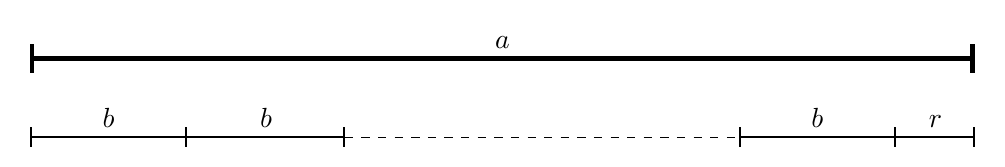
\begin{tikzpicture}
  \draw[|-|, ultra thick] (0,1)--(12,1);
  \node[anchor=south] at (6,1) {$a$};
  \draw[|-|, thick] (0,0)--(2,0);
  \draw[-|, thick] (2,0)--(4,0);
  \draw[dashed] (4,0)--(9,0);
  \draw[|-|, thick] (9,0)--(11,0);
  \draw[-|, thick] (11,0)--(12,0);
  \node[anchor=south] at (1,0) {$b$};
  \node[anchor=south] at (3,0) {$b$};
  \node[anchor=south] at (10,0) {$b$};
  \node[anchor=south] at (11.5,0) {$r$};
\end{tikzpicture}

上图,我们从丈量的角度也理解。能同时丈量$a,b$的线段,都能够量尽$b,r$,反之亦然

带余除法(除法原理)(欧几里得除法Euclidean division)(division with remainder). $a=qb+r, \; 0\le r <|b|$, 可用数学归纳法证明\\
多项式的带余除法(多项式长除法): $A=QB+R$, $R$是零多项式,或者它的次数严格小于$B$的次数

辗转相除法是基于带余除法,进而定义了 欧几里得整环
\subsection{更相减损术}
更相减损术,出自《九章算术》

e.g. $gcd(126, 98)$, 写成分数$\frac{126}{98}$\\
第一步:可半者半之。分子分母约去2,得$\frac{63}{49}$\\
第二步:副置分母、子之数,以少减多,更相减损,求其等也。\\
$(63,49) \rightarrow (14, 49)\rightarrow (14,21) \rightarrow (14,7) \rightarrow (7,7)$

稍加改进,便可以直接计算最大公约数:\\
$(126, 98) \rightarrow (28,98) \rightarrow (28,70)\rightarrow (28,42) \rightarrow (28,14) \rightarrow (14,14)$

与欧几里得的辗转相除相比较,可以把除法看作连续的减法。对于求多个数的最大公因数,更相减损更具优势:
\begin{align*}
  gcd(623, 1424, 801, 1513) &= (623, 1424-801, 801-623, 1513-1424)\\
                            &=(623, 623, 178, 89)\\
                            &= (623-6\times 89, 623 -6\times 89, 178-89, 89)\\
                            &=(89, 89, 89, 89)\\
                            &=89\\
\end{align*}


\section{反证法(proof by contradiction)}
英国数学家高德菲·哈罗德·哈代在他的文章《一个数学家的辩白》描述:“欧几里得最喜欢用的反证法,是数学家最精良的武器。它比起棋手所用的任何战术还要好:棋手可能需要牺牲一只兵甚至更多,但数学家却是牺牲整个棋局来获得胜利。”

反证法常用于“正面证明不容易或不能得出结果”的情况

Procedure:\\
1.The proposition to be proved is $P$\\
2.We assume $P$ to be false, i.e., we assume $\neg P$\\
3.It is shown that $\neg P$ implies falsehood. This is typically accomplished by deriving two mutually contradictory assertions. $Q$ and $\neg Q$ and appealing to the law of noncontradiction\\
4.Since assuming $p$ to be false leads to a contradiction. It's concluded that $p$ is in fact true

Example: $\sqrt{2}$是无理数的证明

假设$\sqrt{2}$是有理数,那么就可以写为$\frac{p}{q}$,其中$p, q$为正整数且互质,那么有: $p=\sqrt{2}\times q$, then $p^2=2\times q^2$, 很显然$p^2$是偶数,而只有偶数的平方才是偶数,所以$p$是偶数。假设$p=2s$,then $p^2=4s^2=2q^2 \Rightarrow q^2=2s^2$, 从而$q$也是偶数,这与互质矛盾,假设不成立,从而得证。

\section{牛顿法(Newton's method, or Newton-Raphson method)}
它是一种在实数域和复数域上近似求解方程的方法

\end{document}
%%% Local Variables:
%%% mode: LaTeX
%%% TeX-master: "../main"
%%% End:
